\documentclass[12pt]{article}

\usepackage{amsmath,amsthm,amssymb,amscd,epsfig,url}
\usepackage{fullpage}
\usepackage{times}
\usepackage{mathdots}
\newtheorem{theorem}{Theorem}[section]
\newtheorem{lemma}[theorem]{Lemma}
\newtheorem{proposition}[theorem]{Proposition}
\newtheorem{corollary}[theorem]{Corollary}
\newtheorem{conjecture}[theorem]{Conjecture}
\newtheorem{definition}[theorem]{Definition}
\newtheorem{example}[theorem]{Example}
\newtheorem{remark}[theorem]{Remark}

\usepackage{xcolor}
\usepackage{tikz}
\usetikzlibrary{arrows.meta, automata, positioning}

\def\ZZ{{\mathbb Z}}
\def\QQ{{\mathbb Q}}
\def\RR{{\mathbb R}}
\def\TT{{\mathcal{C} T}}
\def\KK{{\mathcal{C} K}}
\newcommand{\hus}{\hfill\break}
\newcommand{\bull}{\textbullet\;\;}
\def\iso{{\operatorname{\ \approx \ }}}   % isomorphism
\def\im{{\operatorname{im}}}              % image
\def\Hom{{\operatorname{Hom}}}           % homomorphisms
\def\line{{\operatorname{line} \,}}       % line graph
\def\sd{{\operatorname{sd \,}}}           % first edge subdivision graph
\def\coker{{\operatorname{coker}}}        % cokernel
\def\lcm{{\operatorname{lcm}}}             % least common multiple
\newcommand{\gcdd}{\gamma}              
\def\del{{\partial}}                      % signed incidence matrix
\def\<{{\langle}} \def\>{{\rangle}}       % Inner product
\def\ZC{{Z^\#}}                           % cycle space
\setlength{\textheight}{9in}               
%\setlength{\textwidth}{6in}               % width of text
%\setlength{\oddsidemargin}{0in}           % odd page left margin
%\setlength{\evensidemargin}{0in}          % even page left margin 

\title{Residual Graph Template}
\author{CMSC 27230: Theory of Algorithms}
\date{ }

\begin{document}
\maketitle

\thispagestyle{empty}

\begin{center}
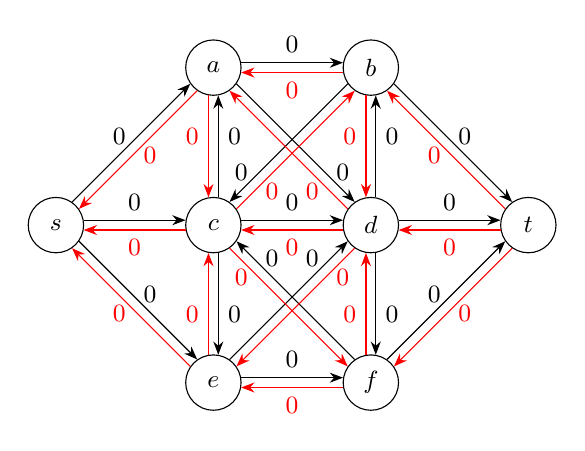
\begin{tikzpicture}[
      mycircle/.style={
         circle,
         draw=black,
         fill=white,
         fill opacity = 0.3,
         text opacity=1,
         inner sep=0pt,
         minimum size=20pt,
         font=\small},
      myarrow/.style={-Stealth},
      node distance=0.6cm and 1.2cm
      ]
      \node[mycircle]  at (-3, 0) (s) {$s$};
      \node[mycircle]  at (-1, 2) (a) {$a$};
      \node[mycircle]  at (1, 2) (b) {$b$};
      \node[mycircle]  at (-1, 0) (c) {$c$};
      \node[mycircle]  at (1, 0) (d) {$d$};
      \node[mycircle]  at (-1, -2) (e) {$e$};
      \node[mycircle]  at (1, -2) (f) {$f$};
      \node[mycircle]  at (3, 0) (t) {$t$};

    \foreach \i/\j/\txt/\p/\pp in {% start node/end node/text/position
      s.55/a.215/0/above/0.4,
      s.10/c.170/0/above/0.5,
      s.325/e.125/0/above/0.6,
      a.10/b.170/0/above/0.5,
      a.325/d.125/0/above/0.9,
      b.215/c.55/0/above/0.9,
      b.325/t.125/0/above/0.6,
	  c.80/a.280/0/right/0.6,
      c.10/d.170/0/above/0.5,
      c.280/e.80/0/right/0.6,
	  d.80/b.280/0/right/0.6,
      d.280/f.80/0/right/0.6,
      d.10/t.170/0/above/0.5,
      e.55/d.215/0/above/0.7,
      e.10/f.170/0/above/0.5,
      f.125/c.325/0/above/0.7,
      f.55/t.215/0/above/0.4
      }
      \draw [myarrow] (\i) -- node[font=\small,\p,pos=\pp] {\txt} (\j);
      \foreach \i/\j/\txt/\p/\pp in {% start node/end node/text/position
      a.235/s.35/0/below/0.4,
      c.190/s.350/0/below/0.5,
      e.145/s.305/0/below/0.6,
      b.190/a.350/0/below/0.5,
      d.145/a.305/0/below/0.3,
      c.35/b.235/0/below/0.3,
      t.145/b.305/0/below/0.6,     
      a.260/c.100/0/left/0.4,
      d.190/c.350/0/below/0.5,
      e.100/c.260/0/left/0.4,    
      b.260/d.100/0/left/0.4,
      f.100/d.260/0/left/0.4,
      t.190/d.350/0/below/0.5,
      d.235/e.35/0/below/0.1,
      f.190/e.350/0/below/0.5,
      c.305/f.145/0/below/0.1,
      t.235/f.35/0/below/0.4
      }
      \draw [myarrow, color = red] (\i) -- node[font=\small,\p,pos=\pp] {\txt} (\j);
\end{tikzpicture}
\end{center}
\end{document}
